\documentclass[twocolumn]{article}
\usepackage[margin=0.75cm]{geometry}
\usepackage{hyperref}
\hypersetup{
    colorlinks,
    citecolor=blue,
    filecolor=blue,
    linkcolor=blue,
    urlcolor=blue
}

\usepackage{graphicx, caption, multirow, mathtools, amsfonts, booktabs, siunitx}
\setlength{\columnseprule}{.75pt}
\def\columnseprulecolor{\color{black}}
\newcommand{\overbar}[1]{\mkern 1.5mu\overline{\mkern-1.5mu#1\mkern-1.5mu}\mkern 1.5mu}

\usepackage{tikz}
\usetikzlibrary{positioning, arrows, fit, decorations.pathmorphing}

\setlength{\parindent}{0pt}
\setlength{\parskip}{6pt}

\everymath{\displaystyle}

\title{
	\vspace{-2em}
	\normalsize \textbf{PHYS 244 Formula Sheet} \\
	\small Eddie Guo \\
	\dotfill
	\vspace{-5em}
}
\date{}

\begin{document}
\maketitle

\small

\textbf{Newtonian Mechanics in Polar Coordinates}

$\hat{r} = \langle \cos \phi, \sin \phi \rangle$ \hfill $\hat{\phi} = \langle -\sin \phi, \cos \phi \rangle$ \hfill $\frac{d\hat{r}}{dt} = \dot{\phi} \hat{\phi}$ \hfill $\frac{d\hat{\phi}}{dt} = -\dot{\phi} \hat{r}$

$\mathbf{r} = r \hat{r}$ \hfill $\mathbf{v} = \dot{r} \hat{r} + r \dot{\phi} \hat{\phi}$ \hfill $\mathbf{a} = (\ddot{r} - r \dot{\phi}^2) \hat{r} + (2 \dot{r} \dot{\phi} + r \ddot{\phi}) \hat{\phi}$

$\dot{\phi} = \omega$ \hfill $\ddot{\phi} = \alpha$ \hfill $v = \omega r$ \hfill $a = \alpha r$

$\begin{cases}
    \sum F_r = m(\ddot{r} - r\dot{\phi}^2) \\
    \sum F_\phi = m(r \ddot{\phi} + 2 \dot{r} \dot{\phi})
\end{cases}$
\hfill
$\begin{cases}
    \text{Centrifugal term:} & -r \dot{\phi}^2 \\
    \text{Coriolis term:} & 2 \dot{r} \dot{\phi}
\end{cases}$

\dotfill

\textbf{Newtonian Mechanics in Cylindrical Coordinates}

$\sum F_\rho = m(\ddot{\rho} - \rho \dot{\phi}^2)$ \hfill $\sum F_\phi = m(\rho \ddot{\phi} + 2 \dot{\rho} \dot{\phi})$ \hfill $\sum F_z = m \ddot{z}$

\dotfill

\textbf{Newtonian Mechanics in Intrinsic Coordinates}

$\mathbf{v} = v \hat{u}_t$ \hfill $\mathbf{a} = \dot{v} \hat{u}_t + \frac{v^2}{r} \hat{u}_n \equiv a_t \hat{u}_t + a_n \hat{u}_n$

$\sum F_t = ma_t$ \hfill $\sum F_n = ma_n = \frac{mv^2}{\rho}$ \hfill $\sum F_b = 0$

$\rho(x) = \frac{(1 + [f'(x)]^2)^{3/2}}{|f''(x)|}$ \hfill $\rho(t) = \frac{| r'(t) |^3}{| r'(t) \times r''(t) |} = \frac{(\dot{x}^2 + \dot{y}^2 )^{3/2}}{|\dot{x} \ddot{y} - \ddot{x} \dot{y}|}$

\dotfill

\textbf{Linear Air Resistance}

\begin{minipage}{0.65\columnwidth}
    $m\mathbf{\ddot{r}} = m \mathbf{g} - b \mathbf{v}$

    \vspace{-.25em} \rule{\columnwidth}{.5pt} \vspace{-.75em}

    $v_x(t) = v_{0x} e^{-bt/m}$ \\[0.5em]
    $v_y(t) = v_{0y} e^{-bt/m} + v_{T,y} (1-e^{-bt/m})$
    
    \rule{\columnwidth}{.5pt} \vspace{-.75em}
    
    $x(t) = x_0 + v_{0x} \tau (1 - e^{-t/\tau})$ \\[0.5em]
    $y(t) = y_0 + (v_{0y} - v_{T,y}) \tau (1-e^{-t / \tau}) + v_{T,y} t$ \\[0.5em]
    $y(x) = \frac{v_{0y} + v_{T,y}}{v_{0x}} x + v_{T, y} \tau \ln \left( 1- \frac{x}{v_{0x}\tau} \right)$ \\[0.5em]
    If $+y$ is up, then flip sign on $v_{T,y}$.
\end{minipage}
\hfill
\begin{minipage}{0.3\columnwidth}
    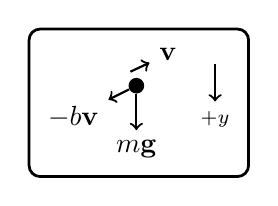
\begin{tikzpicture}[scale=0.8]
        \node (p) [circle, fill, inner sep=2pt] at (0, 0) {};
        \node (f) at (-1, -0.5) {$-b\mathbf{v}$};
        \node (g) at (0, -1) {$m\mathbf{g}$};
        \draw [->, thick] (p) -- (f);
        \draw [->, thick] (p) -- (g);
    
        \node (vp) at (-0.25, 0.15) {};
        \node (v) at (0.5, 0.5) {$\mathbf{v}$};
        \draw [->, thick] (vp) -- (v);

        \node (c1) at (1.25, 0.5) {};
        \node (c2) at (1.25, -0.25) [below] {\scriptsize $+y$};
        \draw [->, thick] (c1) -- (c2);
        
        \node [rectangle, fit = (p) (f) (g) (vp) (v) (c1) (c2), draw=black, line width=1pt, rounded corners] {};
    \end{tikzpicture}

    \vspace{.5em} \flushleft
    $\tau = \frac{m}{b}$ \\[0.5em]
    $v_{T,y} = \frac{mg}{b}$
\end{minipage}

\dotfill

\textbf{Quadratic Air Resistance}

$m \mathbf{\ddot{r}} = m \mathbf{g} - b \mathbf{v}^2$ \hfill $v_T = \sqrt{\frac{mg}{b}}$

$x$-dir only: $v_x(t) = \frac{v_{0x}}{1 + cv_{0x}t/m}$ \hfill $x(t) = \frac{mv_{0x}}{c} \ln \left( 1 + \frac{cv_{0x}t}{m} \right)$

$y$-dir only: $v_y(t) = v_T \tanh \left( \frac{2gt}{v_T} \right)$ \hfill $y(t) = y_0 + \frac{v_T^2}{g} \ln \left( \cosh \frac{gt}{v_T} \right)$

\dotfill

\textbf{Charged Particle in Uniform Magnetic Field}

$\mathbf{F_B} = q \mathbf{v} \times \mathbf{B} = \omega \langle v_y, -v_x \rangle$ \hfill Cyclotron freq: $\omega = \frac{qB}{m}$

$\eta(t) = \eta_0 e^{-i \omega t}$ \hfill $\eta(t) = v_x(t) + i v_y(t)$

$v_x(t) = v_{0x} \cos \omega t + v_{0y} \sin \omega t$ \hfill $v_y(t) = v_{0y} \cos \omega t - v_{0x} \sin \omega t$

$x(t) = x_0 + \frac{v_{0x}}{\omega} \sin \omega t + \frac{v_{0y}}{\omega} (1 - \cos \omega t)$

$y(t) = y_0 + \frac{v_{0y}}{\omega} \sin \omega t - \frac{v_{0x}}{\omega} (1 - \cos \omega t)$

$v_x(t)^2 + v_y(t)^2 = v_{0x}^2 + v_{0y}^2 = v_0^2$

$\left[ x(t) - x_0 - \frac{v_{0y}}{\omega} \right]^2 + \left[ y(t) - y_0 + \frac{v_{0x}}{\omega} \right]^2 = \frac{v_{0x}^2}{\omega^2} + \frac{v_{0y}^2}{\omega^2} = R^2$

\dotfill

\textbf{Linear Momentum}

$\Delta \mathbf{P} = \sum_i \int_0^t \mathbf{F}_{\text{ext},i}\ dt = \mathbf{J}_{\text{net}}$

$e = \frac{v_{b2n} - v_{a2n}}{v_{a1n} - v_{b1n}}$ \hfill $n$-axis is along line of impact, $t$-axis $\perp$ $n$-axis

Geometry known:

\vspace{-.5em}\begin{itemize}
    \item $m_a v_{a1n} + m_b v_{b1n} = m_a v_{a2n} + m_b v_{b2n}$
    \item $v_{a1t} = v_{a2t},\ v_{b1t} = v_{b2t}$
\end{itemize} \vspace{-.5em}

Geometry unknown: conserve total $\mathbf{p}$ in any 2 perpendicular dirs.

\vspace{-.5em}
\dotfill

\textbf{Center of Mass}

$\mathbf{r}_{\text{cm}} = \frac{1}{M} \sum_i m_i \mathbf{r}_i$ \hfill $\mathbf{v}_{\text{cm}} = \dot{\mathbf{r}}_{\text{cm}} = \frac{1}{M} \sum_i m_i \mathbf{v}_i$

$\mathbf{a}_{\text{cm}} = \ddot{\mathbf{r}}_{\text{cm}} = \frac{1}{M} \sum_i m_i \mathbf{a}_i$ \hfill $M\mathbf{a}_{\text{cm}} = \mathbf{F}_{\text{ext,sys}}$

$\mathbf{v}_{b/a} = \mathbf{v}_{b/c} - \mathbf{v}_{a/c}$ \hfill $c$ is an arbitrary inertial frame

Rocket equation: $m \dot{v} = F_{\text{ext,sys}} - v_{\text{ex}} \dot{m}$

$\quad$If $F_{\text{ext,sys}} = 0$: $v(m) = v_0 + v_{\text{ex}} \ln \frac{m_0}{m}$

\dotfill

\textbf{Torque and Angular Momentum}

$\mathbf{l} = \mathbf{r} \times \mathbf{p}$ \hfill $\boldsymbol{\tau} = \mathbf{r} \times \mathbf{F}$ \hfill $\boldsymbol{\tau} = \frac{d\mathbf{l}}{dt}$

Central force: $\mathbf{F} = F(r) \hat{r}$ \hfill $\tau_F = \mathbf{r} \times (F \hat{r}) = 0 \implies \mathbf{l} = \text{const}$

$\quad$Kepler's 2nd law: $\dot{A} = \frac{1}{2} r^2 \dot{\phi} = \frac{l}{2m} \implies A(t) = \frac{l}{2m} t$

$\quad \frac{d\mathbf{L}_0}{dt} = \boldsymbol{\tau}_{\text{ext, sys}}, \quad \boldsymbol{\tau}_{\text{ext, sys}} = I \boldsymbol{\alpha}_z$

$\quad L_z = I_z \omega_z, \quad I_z = \sum_i m_i r_i^2$ or $I_z = \int r^2\ dm$

Parallel axis thm: $I_p = I_{\text{cm}} + Md^2$

$T = \frac{1}{2} I_{\text{cm}} \omega^2 + \frac{1}{2} M v_{\text{cm}}^2$

\dotfill

\textbf{Energy}

$W = \int_{t_1}^{t_2} \mathbf{F}(\mathbf{r}(t)) \cdot d\mathbf{r}(t)$ \hfill WET: $W_{\text{tot}} = \frac{1}{2} m (v_2^2 - v_1^2) = \Delta T$

$W_{\text{g}} = -mg \Delta y = -mg(y - y_0)$

Conservative $\mathbf{F}$: $W_F = -\Delta U = U_1 - U_2$

$\quad \nabla \times \mathbf{F} = 0 \implies \mathbf{F}$ is conservative ($W=0$ on closed path)

$\quad$2D: $\mathbf{F} = P \hat{i} + Q \hat{j} \implies Q_x - P_y = 0 \implies \mathbf{F}$ conservative

$\quad$Option 1: $\mathbf{F} = - \nabla U$ \hfill Option 2: line integral on easy path

If $W_{nc} = 0$, then $\Delta E = 0 \iff \Delta T = -\Delta U$

1D only: $E = \frac{1}{2} mv^2 + U(x)$, then

$\quad v = \pm \sqrt{\frac{2(E-U(x))}{m}} \implies t = \int_{x_0}^x \frac{\pm dx}{\sqrt{2(E-U(x))/m}}$


% new page
\cleardoublepage


$F(x) = -\frac{dU(x)}{dx}$ \hfill Constrained force: $F_s = -\frac{dU}{ds}$

If $dU/dx > 0$, PE $\uparrow$ for increasing $x \implies F < 0$ ($F$ points to $-x$)

If $dU/dx < 0$, PE $\downarrow$ for increasing $x \implies F > 0$ ($F$ points to $+x$)

A central force is conservative iff it's spherically symmetric.

$\quad \mathbf{F}_{\text{central}} = f(\mathbf{r}) \hat{r} = f(r, \phi, \theta) \hat{r}$

$\quad$Spherically symm: $f(r, \phi, \theta) \mapsto f(r)$

$U_{\text{int, sys}} = \sum_i \sum_{j>i} U_{ij}$

Mech energy: $E = \sum_i \frac{1}{2} m_i v_i^2 + \sum_i \sum_{j > i} U_{ij} + \sum_i U_{i, \text{ext}}$

$W_{\text{non-cons}} = -\Delta U_{\text{int}}$ \hfill $\sum_{\text{universe}} (K + U + U_{\text{int}}) = \text{const}$

\dotfill

\textbf{Oscillations}

$U(x) \approx \frac{1}{2} U''(0) x^2 + \frac{1}{3!} U'''(0) x^3 + \cdots$

$\quad k := U''(0)$ \hfill $k > 0$ for stable eq

$\ddot{x}(t) + \omega^2 x(t) = 0$ \hfill $\omega = \sqrt{k/m}$

\vspace{-.5em}
\dotfill

\textit{Coupled Oscillators}

\begin{figure}[h!]
    \centering
    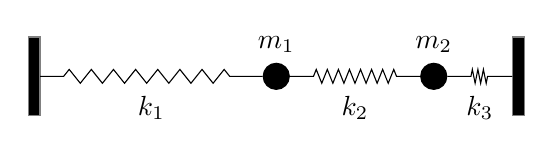
\begin{tikzpicture}[
        wall/.style = {gray,fill=black},
        mass/.style = {draw,circle, fill=black},
        spring/.style = {decorate,decoration={zigzag, pre length=.3cm,post length=.3cm,segment length=#1}},
        ]
        \draw[wall] (-.15,-0.5) rectangle (0,0.5);
        \coordinate (l) at (0,0);
        \node[mass,label={above:$m_1$}] (m1) at (3,0) {};
        \node[mass,label={above:$m_2$}] (m2) at (5,0) {};
        \coordinate (r) at (6,0);
        \draw[wall] (6,-.5) rectangle (6.15,.5);
    
        \draw[spring=8pt] (l) -- node[below, yshift=-.35em] {$k_1$} (m1);
        \draw[spring=4pt] (m1) -- node[below, yshift=-.35em] {$k_2$} (m2);
        \draw[spring=2pt] (m2) -- node[below, yshift=-.35em] {$k_3$} (r);
    \end{tikzpicture}
\end{figure}

$\begin{bmatrix} m_1 & 0 \\ 0 & m_2 \end{bmatrix} \begin{bmatrix} \ddot{x}_1 \\ \ddot{x}_2 \end{bmatrix} = \begin{bmatrix} -k_1-k_2 & k_2 \\ k_2 & -k_2 - k_3 \end{bmatrix} \begin{bmatrix} x_1 \\ x_2 \end{bmatrix}$ \hfill $\implies$ \hfill $\mathbf{M} \ddot{\mathbf{x}} = -\mathbf{K} \mathbf{x}$

$\quad \implies -\omega^2 \mathbf{M} (\mathbf{a} e^{i \omega t}) = -\mathbf{K} (\mathbf{a} e^{i \omega t}) \implies \det(\mathbf{K} - \omega^2 \mathbf{M}) = 0$

\vspace{-.5em} \begin{enumerate}
    \item Find characteristic equation and solve for eigenvalues.
    \item Plug eigenvalues back to solve for eigenvectors.
    \item $\mathbf{z}_i(t) = A_i (\text{eigval}) (\text{eigvec}) e^{i(\omega_i t - \delta_i)} = C_i (\text{eigval}) (\text{eigvec}) e^{i\omega_i t}$.
    \item $\mathbf{x}(t) = \text{Re} \{ \mathbf{z}(t) \}$. Each $\mathbf{x}_i(t)$ is a normal mode.
\end{enumerate} \vspace{-.5em}

\vspace{-.5em}
\dotfill

\textit{Case 1: $m_1 = m_2,\ k_1 = k_2 = k_3$}

$\mathbf{x}_1(t) = A_1 \begin{bmatrix} 1 \\ 1 \end{bmatrix} \cos(\omega_0 t - \delta)$ \hfill $\mathbf{x}_2(t) = A_2 \begin{bmatrix} 1 \\ -1 \end{bmatrix} \cos(\sqrt{3} \omega_0 t - \delta)$

$\quad \omega_0 = \sqrt{\frac{k}{m}}$

\dotfill

\textit{Case 2: $m_1 = m_2,\ k_2 \ll k_1 = k_3 = k$}

$\mathbf{x}(t) = \left( C_1 \begin{bmatrix} 1 \\ 1 \end{bmatrix} e^{i \epsilon t} + C_2 \begin{bmatrix} 1 \\ -1 \end{bmatrix} e^{-i \epsilon t} \right) e^{i \omega_{\text{avg}} t}$

$\quad \omega_1 = \sqrt{\frac{k+2k_2}{m}} = \omega_{\text{avg} + \epsilon}$ \hfill $\omega_2 = \sqrt{\frac{k}{m}} = \omega_{\text{avg} - \epsilon}$

$\quad \omega_{\text{avg}} = \frac{\omega_1 + \omega_2}{2}$ \hfill $\epsilon = \frac{\omega_2 - \omega_1}{2} \ll \omega_{\text{avg}}$

If $C_1 = _2 = \frac{A}{2}$, then $\mathbf{z}(t) = A \begin{bmatrix} \cos \epsilon t \\ i \sin \epsilon t \end{bmatrix} (\cos \omega_{\text{avg}}t + i \sin \omega_{\text{avg}} t)$.

$\quad \mathbf{x}(t) = \text{Re} \{ \mathbf{z}(t) \} = A \begin{bmatrix} \cos\epsilon t \cos \omega_{\text{avg}} t \\ -\sin \epsilon t \sin \omega_{\text{avg}} t \end{bmatrix} \implies$ beats


% new page
\newpage


\textbf{Linear Damped SHO}

$m\ddot{x} = -kx - b\dot{x} \implies \ddot{x} + 2\beta\dot{x} + \omega_0^2 x = 0$ \hfill $2 \beta = \frac{b}{m},\ \omega_0^2 = \frac{k}{m}$

$\hat{D} = \frac{d^2}{dt^2} + 2 \beta \frac{d}{dt} + \omega_0^2 \implies \hat{D} x = 0$

$\quad \beta > \omega_0 \implies x(t) = C_1 e^{- \left(\beta + \sqrt{\beta^2 - \omega_0^2} \right) t} + C_2 e^{-\left(\beta - \sqrt{\beta^2 - \omega_0^2} \right) t}$

$\quad \beta = \omega_0 \implies x(t) = e^{-\beta t} (C+Dt)$

$\quad \beta < \omega_0 \implies x(t) = e^{-\beta t} (A \cos \omega_d t + B \sin \omega_d t),\ \omega_d = \sqrt{\omega_0^2 - \beta^2}$

\vspace{-.5em}
\dotfill

$\hat{D} x =  f_0 \cos \omega t$ \hfill $f_0 = \frac{F_{\text{max}}}{m},\ \beta = -\frac{b}{2m},\ \omega_0 = \sqrt{\frac{k}{m}}$

$\quad x_p(t) = \underbrace{\frac{f_0}{\sqrt{(\omega_0^2 - \omega^2)^2 + 4 \beta^2 \omega^2}}}_{A(\omega)} \cos(\omega t - \delta)$

$\quad A(\omega)$ is a Lorentzian fn \hfill $\omega_{\text{max}} = \sqrt{\omega_0^2 - 2 \beta^2}$

\vspace{-.5em}
\dotfill

\textbf{Lagrangian Mechanics}

$L = T - U,\quad L = L(q, \dot{q}, t)$

$S = \int_{t_1}^{t_2} L(q, \dot{q}, t)\ dt \implies \frac{\partial L}{\partial q_i} = \frac{d}{dt} \left( \frac{\partial L}{\partial \dot{q}_i} \right)$

\vspace{-.5em} \begin{itemize}
    \item If $F(y, y', x) = F(y', x)$, then $\frac{\partial F}{\partial y'} = \text{const}$
    \item Beltrami identity: $F - y' \frac{\partial F}{\partial y'} = C$
\end{itemize} \vspace{-.5em}

$L = T - U,\ \frac{d}{dt} \left( \frac{\partial L}{\partial \dot{x}_i} \right) = \frac{\partial L}{\partial x_i} \iff m \ddot{x}_i = -\frac{\partial U}{\partial x_i}$

Hamilton's principle: $\delta S = \delta \int_{t_0}^{t_f} L\ dt = 0$

$\frac{d}{dt} (\text{generalized momentum}) = \text{generalized force}$

If E-L eq holds for $x_i = x_i(q_1, q_2, \dots, q_n; t)$, then it also holds for the $q_i$ coordinates. That is,

$\quad \frac{d}{dt} \left( \frac{\partial L}{\partial \dot{q}_m} \right) = \frac{\partial L}{\partial q_m}, \quad 1 \leq m \leq n$

Constraint forces are automatically incorporated with the right choice of generalized variables.

\vspace{-.5em}
\dotfill

\textit{Generalized Coordinates and Degree of Freedom}

Parameters $\{ q_1, \dots, q_n \}$ called a set of generalized coordinates if $\mathbf{r}_\alpha = \mathbf{r}_\alpha(q_1, \dots, q_n, t)$ and $q_i = q_i (\mathbf{r}_1, \dots, \mathbf{r}_n, t)$ s.t. $n$ is the smallest number that allows the system to be parameterized this way.

Natural coordinates: relation btw $\mathbf{r}$ and $q$ is time-indep

Dof: coordinate that can be varied indep of others

Holonomic sys: $\# \text{dof} = \# \text{generalized coordinates}$

\vspace{-.5em}
\dotfill

\textit{Conservation Laws}

Spatial translational invariance $\iff$ cons of total momentum

Time translational invariance $\iff$ cons of $E$ \hfill (think Beltrami)

Hamiltonian: $H = \left( \sum_i \dot{q}_i \frac{\partial L}{\partial \dot{q}_i} \right) - L$

$\quad H$ is the Legendre transform of $L$


\cleardoublepage


\begin{enumerate}
    \item If the relation btw generalized coords $q_i$ and Cartesian coords is time-indep, then $H$ is the $E$ of the sys.
    \item If $L$ as no explicit time dependence, then $H$ is conserved.
\end{enumerate} \vspace{-.5em}

\textit{Noether's thm}. For each continuous symmetry of $L$, there is exists a conserved quantity.

$\quad$Noether charge/cons of gen $p$: $Q_{\text{cons}} = \sum_i \frac{\partial L}{\partial \dot{q}_i} K_i$

$\quad K_i(q)$ are called generators of symmetry.

\vspace{-.5em}
\dotfill

\textit{Lagrange Multipliers and Constraint Forces}

$\frac{d}{dt} \left( \frac{\partial L}{\partial \dot{q}_i} \right) = \frac{\partial L}{\partial q_i} + \lambda(t) \frac{\partial f}{\partial q_i}$ \hfill $\lambda(t)$ is the Lagrange multiplier
 
$f(q_1, q_2) = c, \quad f$ is a constraint

\vspace{-.5em}
\dotfill

\textbf{Two-Body Central Force Problems}

$\mathbf{r} = \mathbf{r}_1 - \mathbf{r}_2$ \hfill $\mathbf{R} = \frac{m_1\mathbf{r}_1 + m_2\mathbf{r}_2}{M}, \quad M = m_1 + m_2$

$\mathbf r_1 = \mathbf R + \frac{m_2}{M} \mathbf r$ \hfill $\mathbf r_2 = \mathbf R - \frac{m_1}{M} \mathbf r$

Reduced mass: $\mu = \frac{m_1 m_2}{m_1 + m_2} = \frac{m_1 m_2}{M}$

$L = \frac{1}{2} M\dot{\mathbf{R}}^2 + \frac{1}{2} \mu \mathbf{\dot{r}}^2 - U(r)$

$\mu \ddot r = -\frac{dU}{dr} + \frac{l_z^2}{\mu r^3}$ \hfill $U_{\text{eff}}(r) = U(r) + \frac{l_z^2}{2\mu r^2}$

\dotfill

\textit{Inverse Square Law}

$U_{\text{eff}}(r) = -\frac{\gamma}{r} + \frac{l_z^2}{2 \mu r^2}$ \hfill $F(r) = -\frac{\gamma}{r^2} \iff U(r) = -\frac{\gamma}{r}$

$\frac{dU_{\text{eff}}}{dt} = 0 \implies r_0 = \frac{l_z^2}{\gamma \mu}$ \hfill $\frac{d^2 U_{\text{eff}}}{dt^2} = \frac{\gamma^4 \mu^3}{l_z^6} > 0,\ \gamma > 0$

$\quad E < 0$: particle bound \hfill $E > 0$, particle unbound ($r \to \infty$)

$U(r) = -\frac{\gamma}{r} \implies r(\phi) = \frac{c}{1+\epsilon \cos \phi}$ \hfill $c = \frac{l_z^2}{\gamma \mu},\quad \epsilon = \frac{Al_z^2}{\gamma \mu}$

$E = \frac{\gamma^2 \mu}{2l_z^2} (\epsilon^2 - 1)$

\dotfill

\textit{Equation for Orbits}

$\mu \ddot{r} = -\frac{\gamma}{r^2} + \frac{l_z^2}{\mu r^3}$

$\quad \dot r = \sqrt{\frac{2[E-U_{\text{eff}}(r)]}{\mu}} \implies t = \int_{r_0}^{r} \frac{dr}{\sqrt{2 [E-U_{\text{eff}}] / \mu}}$

$\quad \phi - \phi_0 = \frac{l_z}{\mu} \int_0^t \frac{dr}{[r(t)]^2}$

\textit{We can do better (i.e., linearize the ODE)!}

$w \equiv \frac{1}{r} \implies \frac{d^2 w}{d\phi^2} = \frac{\gamma \mu}{l_z^2} - w$

$w(\phi) = A \cos(\phi - \phi_0) + \frac{\gamma \mu}{l_z^2} = \frac{\gamma \mu}{l_z^2} \left[ 1 + A \frac{l_z^2}{\gamma \mu} \cos(\phi-\phi_0) \right]$

Let $c = \frac{l_z^2}{\gamma \mu}$ and $\epsilon = \frac{Al_z^2}{\gamma \mu}$ and choose polar axes st $\phi_0 = 0$

$\implies w(\phi) = \frac{1+\epsilon \cos \phi}{c} \implies r(\phi) = \frac{1}{1+\epsilon \cos \phi}$


\newpage


Bound states ($E < 0$): $\epsilon = 0$: circle, $0 < \epsilon < 1$: ellipse

Unbound states ($E \geq 0$): $\epsilon = 1$: parabola, $\epsilon > 1$: hyperbola

$\frac{1}{2} \mu \dot r^2 + U_{\text{eff}}(r) = E \implies E = U_{\text{eff}}(r_{\text{min}}) = -\frac{\gamma}{r_{\text{min}}} + \frac{l_z^2}{2 \mu r^2_{\text{min}}}$

$\quad r_{\text{min}} = \frac{c}{1+\epsilon} \implies E = \frac{\gamma^2 \mu}{2l_z^2} (\epsilon^2-1)$

\dotfill

\textbf{Hamiltonian Mechanics}

$H = H(q_i, p_i)$ \hfill $\dot q_i = \frac{\partial H}{\partial p_i}$ \hfill $\dot p_i = -\frac{\partial H}{\partial q_i}$

$H = \sum_i \frac{\partial L}{\partial \dot q_i} \dot q_i - L = \sum_i p_i \dot q_i - L$

$H = T + U$ if $q_i$ are time-indep

\begin{enumerate}
    \item Choose suitable generalized coords $q_i$.
    \item Det $T$ and $U$ in terms of $q_i$ and $\dot q_i$.
    \item Det $p_i$. If sys conservative, $p_i = \partial T / \partial \dot q_i$.
    \item Solve for $\dot q_i$ in terms of $p$ and $q$.
    \item Write down $H$ and 1st order Hamiltonian eqs of motion.
\end{enumerate}


\end{document}
